% !TEX root = ../main.tex
\chapter{建模与仿真}

\section{求解过程的简述}
根据第二章中推导的反应过程,仿真的过程主要分为以下三步:

1)在COMSOL Multiphysics中,对通电时发生的电化学反应进行建模,得到阴极极板表面的平均$\ce{OH-}$浓度随
时间的变化曲线。

2)利用第1步得到的浓度变化随时间的变化曲线,在MATLAB中计算$\ce{Zr^4+}$的水解程度随时间的变化关系,
再根据$\ce{Zr^4+}$消耗与DNA释放这一正比关系,得到DNA的释放曲线。

3)利用第2步得到的数据,在COMSOL Multiphysics中,对DNA在电场力以及浓度梯度力作用下的扩散、迁移过程进行建模仿真。
\section{反应容器物理模型}
本课题组使用的反应容器为一个长度为$2cm$,直径为$1cm$的圆柱体。作为电极的金薄膜的规格为$20mm×6mm×1mm$。

如图~\ref{fig:container} 所示,根据上述数据,我们可以在COMSOL Multiphysics中完成对反应溶液的物理模型的建立。
由于电极材料为金,不参与反应,内部也考虑为等势体,所以我们只用考虑在溶液体系内发生的反应,在建模时只用对溶液
进行建模。
\begin{figure}[ht]
    \centering
    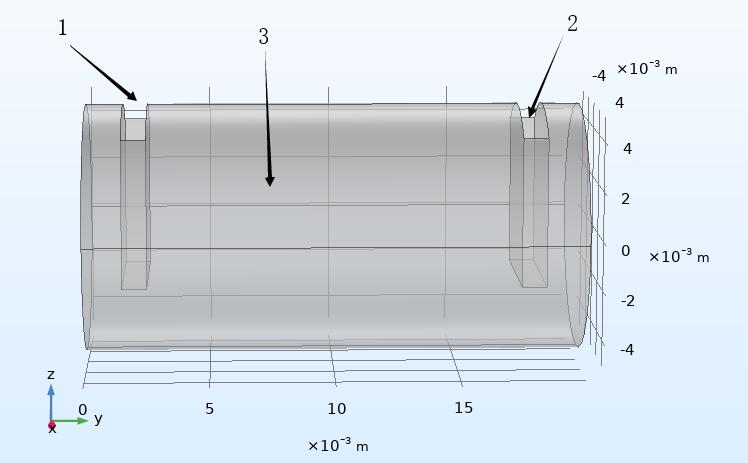
\includegraphics[scale=1]{container.jpg}\\
    1)阳极(Anode) 2)阴极(Cathode) 3)电解液(Electrolyte)
    \caption{反应容器物理模型}
    \label{fig:container}
\end{figure}

\section{电化学反应仿真}
\subsection{计算流程}
——介绍COMSOL Multiphysics的操作及计算过程
\subsection{结果与讨论}
——讨论结果以及参数影响等

\section{Zr$^{4+}$水解反应仿真}
\subsection{计算流程}
——介绍在MATLAB中计算水解量
\subsection{结果与讨论}
——讨论结果以及参数影响等

\section{DNA扩散过程仿真}
\subsection{计算流程}
——介绍COMSOL Multiphysics的操作及计算过程
\subsection{结果与讨论}
——讨论结果以及参数影响等